To test the stability of Euler forward (Euler) and the velocity-Verlet (VV) method, we initialize the Earth-Sun system with a circular orbit as stated in Algorithms \ref{alg::euler,alg::verlet}.

We varies the step size $h$ starting from 0.02 yr to 0.001 yr.
The Earth's orbits calculated by these two methods for 10 years are show in Fig. \ref{fig::earth}. 
Globally speaking, we see orbits given by the Euler method expand in time.  
On the other hand, VV methods' orbits keep circular with some tiny fluctuation hardly seen in Fig. \ref{fig:earth500}.
It justifies the our statements in Sec. \ref{method} that the VV method conserves energy but the Euler method increase energy.

For a large step size in Fig. \ref{fig:earth500}, the Euler method is very unstable. Its orbit deviates from circle both in distance and shape apparently. 
As the step size becomes smaller, we can see that the Euler method becomes better; as the orbits expand slower and slower from \ref{fig:earth500} to Fig. \ref{fig:earth10000}.
 The trends we observed agree with the statement that the error in the Euler method goes down with decreasing $h$. We can hardly see differences between orbits yielded from the VV method, which indicates the it's stability.
 
\begin{figure}[tb]
	\begin{subfigure}[tb]{0.5\textwidth}
		\centering
		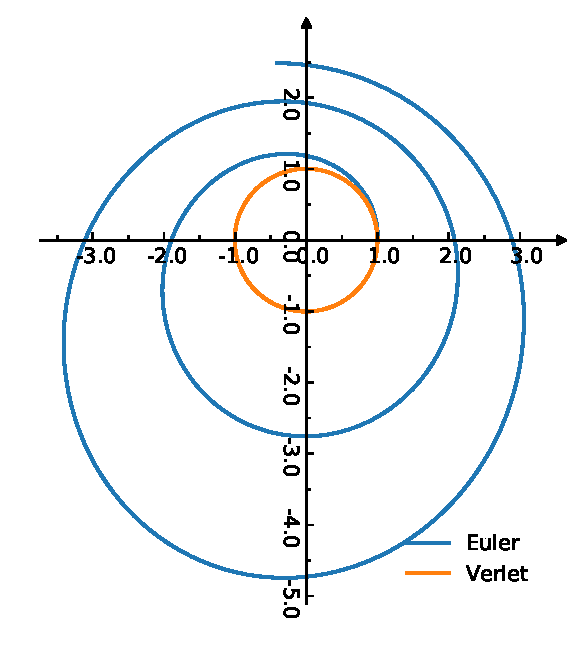
\includegraphics[width=0.7\textwidth]{Earth500.eps}
		\caption{$h = 0.02$yr}
		\label{fig:earth500}
	\end{subfigure}
~
	\begin{subfigure}[tb]{0.5\textwidth}
		\centering
		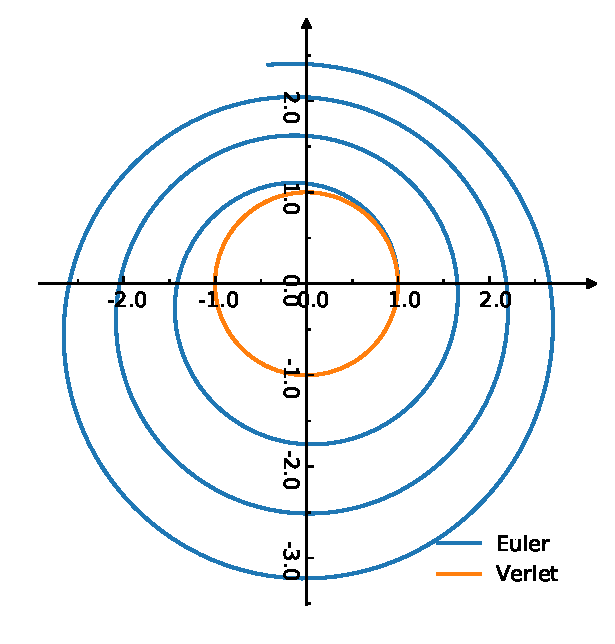
\includegraphics[width=0.7\textwidth]{Earth1000.eps}		\caption{$h = 0.01$year}
		\label{fig:earth1000}
	\end{subfigure}
~
	\begin{subfigure}[tb]{0.5\textwidth}
		\centering
		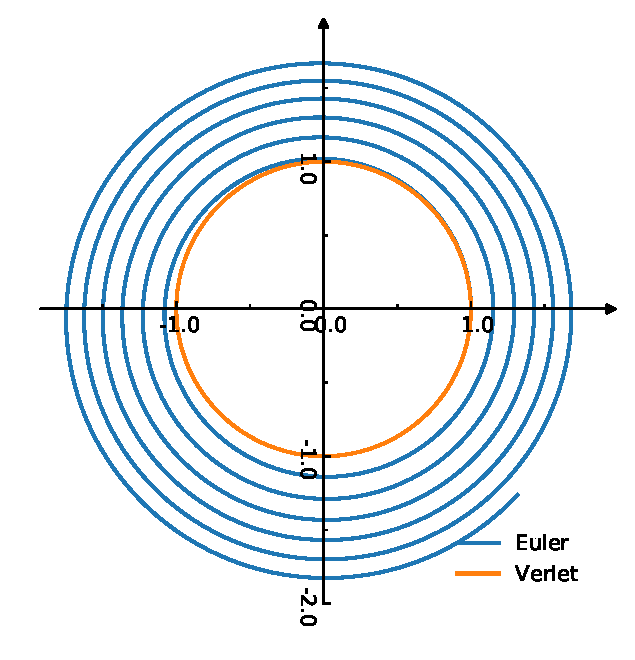
\includegraphics[width=0.7\textwidth]{Earth5000.eps}		\caption{$h = 0.002$year}
		\label{fig:earth5000}
	\end{subfigure}
~
	\begin{subfigure}[tb]{0.5\textwidth}
		\centering
		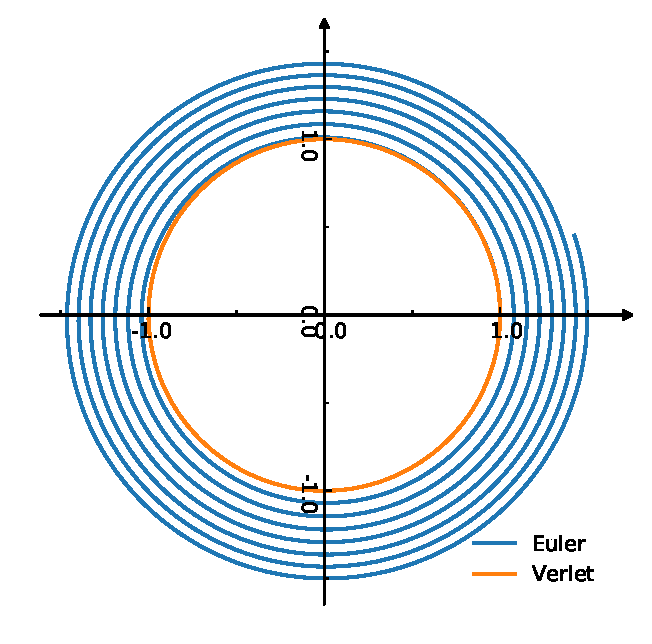
\includegraphics[width=0.7\textwidth]{Earth10000.eps}		\caption{$h = 0.001$year}
		\label{fig:earth10000}
	\end{subfigure}
	\caption{Comparison of different step size $h$ of two methods for 10 years. }
	\label{fig::earth}
\end{figure}

 For detailed check and performance comparison, we list distances, energies, angular momentums together with execution times for these two methods in Table \ref{tab::euler}\&\ref{tab::verlet} with precision up to $10^{-6}$.
 As conservation laws predicted by classical mechanics, physical quantities including kinetic, potential, total energies and angular momentum should be conserved in the Earth-Sun system. 
 From these two tables, we can see conservations in the VV method but not in the Euler method. Thus, we can conclude that the VV method is stable and the Euler method is not.
 
 Compared the execution time of two methods, we find the Euler method is faster. 
 Counting the FLOPS from these two algorithms, we find there is  about 30$N$ for the Euler method and 45$N$ for the VV method. It explains speed advantage of the Euler method.
 
\begin{table}[tb]
	\centering
	\caption{The Euler forward method: step size; kinetic energy; potential energy; total energy; angular momentum in z direction, distance from the Sum and execution time from left to the right.}
	\label{tab::euler}
	\begin{tabular}{ccccccc}
	\hline
	\hline
$h$          & $E_{kin}$        & $E_{pot}$         & $E_{tot}$          & $L_z$        & $r$         & execution time (ms)         \\
	\hline
2.000E-02 & 3.300E-05 & -4.700E-05 & -1.400E-05 & 3.500E-05 & 2.520E+00 & 2.500E-02 \\
1.000E-02 & 2.900E-05 & -4.900E-05 & -2.000E-05 & 3.200E-05 & 2.432E+00 & 5.000E-02 \\
2.000E-03 & 3.200E-05 & -6.500E-05 & -3.300E-05 & 2.500E-05 & 1.824E+00 & 9.400E-02 \\
1.000E-03 & 4.000E-05 & -7.900E-05 & -4.000E-05 & 2.300E-05 & 1.493E+00 & 1.680E-01\\
	\hline
	\hline
\end{tabular}
\end{table}

\begin{table}[tb]
	\centering
	\caption{The Velocity-Verlet method: step size; kinetic energy; potential energy; total energy; angular momentum in z direction, distance from the Sum and execution time from left to the right.}
	\label{tab::verlet}
	\begin{tabular}{ccccccc}
	\hline
	\hline
$h$          & $E_{kin}$        & $E_{pot}$         & $E_{tot}$          & $L_z$        & $r$         & execution time (ms)         \\
	\hline
2.000E-02 & 5.900E-05 & -1.180E-04 & -1.180E-04 & 1.900E-05 & 1.000014 & 2.600E-02 \\
1.000E-02 & 5.900E-05 & -1.180E-04 & -1.180E-04 & 1.900E-05 & 1.000E+00 & 5.600E-02 \\
2.000E-03 & 5.900E-05 & -1.180E-04 & -1.180E-04 & 1.900E-05 & 1.000E+00 & 1.840E-01 \\
1.000E-03 & 5.900E-05 & -1.180E-04 & -1.180E-04 & 1.900E-05 & 1.000E+00 & 3.350E-01\\
	\hline
	\hline
\end{tabular}
\end{table}

For physically meaningful, we will keep using the VV method in our further calculations.